% Capítulo 7. Directores y control automático de vuelo
% 7.1      Indicador director de actitud, Indicador de situación horizontal.
% 7.2      Componentes y modos del director de vuelo, diagrama en bloque, flujo de señales.
% 7.3      Piloto automático, componentes, diagrama en bloque, funcionamiento en los distintos modos.


\chapter{Directores y control autom\'atico de vuelo}
\label{chap:U07.director.vuelo}

\section{Introducci\'on}
\label{sec:07.00.introduccion}

Estos sistemas tienen como finalidad guiar al piloto para que \'este efect\'ue en forma correcta las maniobras de vuelo seg\'un el modo de operaci\'on elejido, adem\'as cumple las funciones b\'asicas de indicaci\'on de actitud y rumbo.

En escencia un Director de Vuelo, en ingl\'es \ac{FDS}, es un sistema de Piloto Autom\'atico sin los servos. El sistema efect\'ua los mismos c\'alculos y sensados que el Piloto Autom\'atico pero es el Piloto quien controla la aeronave y realiza las maniobras siguiendo las instrucciones del panel de control. Varios sistemas de Piloto Autom\'atico disponen la posibilidad de acoplar o desacoplar al \ac{FDS}.

Existen diferentes tipos de \ac{FDS} en cuanto a la forma de 
indicaci\'on y selecci\'on de modos pero cumplen la misma funci\'on. Para la descripci\'on de un sistema t\'ipico se emplear\'a el provisto por la empresa Sperry el Sperry Three Axis Attitude Reference System (STARS), desarrollado en los a\~nos 1960. Se lo suele encontrar en aviones comerciales y particulares donde se integran con los Pilotos Autom\'aticos.


\section{Componentes de cabina}
\label{sec:componentes.cabina}

Un \ac{FDS} puede emplear una o dos pantallas, o estar integrada a otro sistema de presentaci\'on de datos. 
La primera presenta un conjunto de barras de comando, una horizontal y otra vertical. Las barras de comando en esta configuración se mantienen en una posición centrada. 
La segunda usa un avión en miniatura alineado a una señal de comando.

\begin{figure}[!h]
  \centering
    \includegraphics[width=0.75\textwidth]{07.directores.y.ctrol.automatico.vuelo/imagenes/adi+hsi+computador_presentacion.png}  
  \caption{Componentes t\'ipicos de un \ac{FDS}. Arriba a la izquierda el ADI, abajo a la izquierda el HSI, abajo a la derecha la Computadora de Control. (Gentileza Sperry) }
  \label{fig:07.componentes.tipico.FDS.sperry-STARS}
\end{figure}


\subsection{Indicador y Director de Actitud }
\label{sec:adi}

El \ac{ADI} 
 posee una esfera indicadora de actitud y punteros de 
mando (lateral y vertical), que dan al piloto la informaci\'on requerida
para interceptor y mantener una determinada senda de vuelo que, junto
con sus dem\'as componentes, son:

\begin{figure}[!h]\centering
  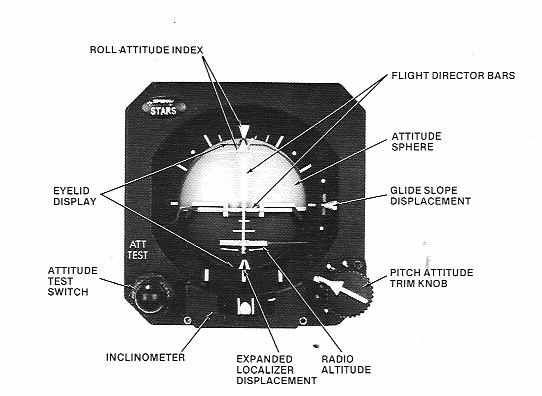
\includegraphics[width=0.98\textwidth]{07.directores.y.ctrol.automatico.vuelo/imagenes/adi.png}
  \caption{Imagen de ADI (gentileza Sperry)}
\label{fig:07.adi.sperry}
\end{figure}

\begin{itemize}
	\item {\bf Esfera de actitud: } parte m\'ovil donde est\'a simbolizado
	el horizonte terrestre, sus movimientos con respecto a un avi\'on simb\'olico
	fijo, indican la actitud en alabeo y cabeceo de la aeronave.

        \item {\bf Avi\'on simb\'olico en miniatura: } s\'imbolo fijo al centro del
	instrumento y con respecto a su centro dan su indicaci\'on las barras de mando, 
	adem\'as de cumplir la funci\'on indicada en el punto anterior.

        \item {\bf Indice de actitud en alabeo: } se mueve con la esfera indicando
	exactamente las gradas en esta actitud.

        \item {\bf Barras de mando: } su funci\'on es dirigir al piloto para interceptar
	y mantener una predeterminada senda de vuelo con la condici\'on de ``volar''
	el peque\~no avi\'on simb\'olico hacia las barras de comando y tratar de
	mantener el centro de este en la intersecci\'on de las barras.
	La barra de mando vertical comanda las actitudes a tomar en alabeo y la
	horizontal en cabeceo.
	Dado que el ``avi\'on'' es fijo, al tomar la actitud correcta las barras que
	son m\'oviles se posicionar\'an en el centro de este s\'imbolo.

        \item {\bf Escala de senda de planeo: }
	el \'indice muestra la desviaci\'on del avi\'on del centro del haz de senda de 
	planeo (Glide Slope) cuando es sintonizada la frecuencia del ILS y la se\~nal
	recibida es v\'alida. 
	Si el avi\'on est\'a volando por debajo del haz, el \'indice se ubicar\'a
	en la parte de arriba de la escala.
	Una indicaci\'on al punto del \'indice representa, aproximadamente,
	 una desviaci\'on de 0,4º
	respecto de la l\'inea de control del haz.

        \item {\bf Barra de radio altura: }
	con el sistema de radioalt\'imetro en funcionamiento, esta barra aparece
	a la vista a los 61 m de altura respecto al terreno, movi\'endose hacia el
	avi\'on en miniatura seg\'un se desciende 

        \item {\bf Localizador expandido: }
	provee de una muy sensible indicaci\'on de la posici\'on del avi\'on
	respecto a la linea central del localizador, siendo utilizado en la
	aproximaci\'on final, dada su sensibilidad.

        \item {\bf Inclin\'ometro: }
	suministra al piloto una indicaci\'on convencional de los deslizamientos
	y derrapes del avi\'on. Al mantener la esfera indicadora centrada,
	se aseguran maniobras coordinadas.

        \item {\bf Perilla de ajuste de actitud de cabeceo: }
	permite posicionar la barra horizontal para que esta comande una
	predeterminada actitud de cabeceo durante una picada o trepada.

        \item {\bf Pulsador de prueba de actitud: }
	opera como una autoprueba del indicador de actitud. Cuando es pulsada
	la esfera se posiciona arrastrando un alabeo de 20º a la derecha
	y un cabeceo de 10º en trepada, apareciendo en este caso una bandera
	de advertencia de actitud erronea.

        \item {\bf Llave de erecci\'on r\'apida del gir\'oscopo: }
	no se encuentra sobre el instrumento, ubic\'andose en el tablero.
	Cuando esta, que es cargada a resorte, es pulsada y mantenida, 
	permite la erecci\'on del gir\'oscopo a una velocidad, aproximada,
	de 2º/minuto, cuando este gire a su m\'axima velocidad.
	Esta llave debe ser accionada cuando el avi\'on se encuentra
	nivelado, y se utiliza en caso de que el gir\'oscopo haya salido
	de su plano de referencia, como puede ocurrir por haberse tomado
	actitudes que superan las posibilidades del sistema.

\end{itemize}

\subsection{Indicador de Situaci\'on Horizontal}
\label{sec:indicador.situacion.horizontal}

El \ac{HSI} 
 provee adem\'as de la indicaci\'on de rumbo del avi\'on
una indicaci\'on pictogr\'afica que representa la posici\'on
de la aeronave respecto a un localizador VOR, y una indicaci\'on de la
posici\'on del avi\'on respecto a la senda de planeo.

\begin{figure}[!h]
  \centering
  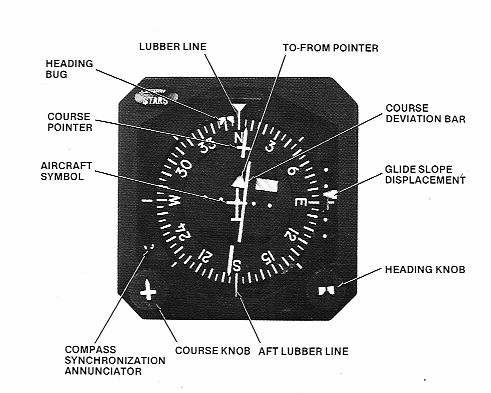
\includegraphics[width=0.98\textwidth]{07.directores.y.ctrol.automatico.vuelo/imagenes/hsi.png}  
  \caption{Imagen HSI (gentileza Sperry)}
  \label{fig:07.hsi.sperry}
\end{figure}


La descripci\'on de cada uno de sus componentes:

\begin{itemize}
	\item {\bf S\'imbolo del avi\'on:} se encuentra fijo e indica la
		posici\'on de la aeronave respecto a un curso de radio
		y a un cuadrante m\'ovil indicador del rumbo. Esta fijado
		al vidrio del instrumento.

        \item {\bf Cuadrante rotante de rumbo:} provee ula informaci\'on de un
	comp\'as magn\'etico girosc\'opico, girando seg\'un los rumbos tomados por
	la aeronave a trav\'es de los 360º.

        \item {\bf Indice principal de rumbo: } 
	es fijo y marca sobre el cuadrante el rumbo del avi\'on.

        \item {\bf Marcas de azimut: }
	se encuentran fijas a una diferencia de 45º a trav\'es de los 360º

        \item {\bf Indice y perilla de rumbo selectado: }
	por medio de la perilla se posiciona el \'indice en la carta al rumbo
	deseado. La diferencia angular entre el rumbo del avi\'on y el preselectado
	

        \item {\bf Puntero y perilla de curso: } este se osiciona en el cuadrante de 
	rumbo por medio de la perilla de curso de manera que
	coincida con el radial de VOR o curso de localizador deseado.
	Igual que el \'incide de rumbo selectado, el puntero de curso es posicionado
	sin afectar la indicaci\'on del cuadrante de rumbo, pero al girar este
	lo hace de igual forma.
	El puntero provee en forma continua la informaci\'on del error de curso
	al piloto y a la computadora del sistema, de manera que 
	cuando es selectado un modo de radio, la barra vertical en el ADI
	dirije al piloto para que controle los comandos y asuma las actitudes
	de alabeo que lo llevar\'an a interceptar y mantener el curso de radio
	selectado, todo esto con la condici\'on de matener la barra vertical en el 
	ADI centralizada.

      \item {\bf Barra de desviaci\'on de curso: }
	representa la l\'inea central del curso selectado de VOR o localizador, 
	el s\'imbolo del avi\'on muestra la posici\'on relativa del mismo
	respecto al curso selectado. Esta barra se mueve paralelamente al puntero
	de curso seg\'un la se\~nal de radio recibida.

      \item {\bf Puntos de desviaci\'on de curso: }
	en la operaci\'on de VOR, cada punto representa 5º de desviaci\'on de la l\'inea
	central y en ILS, es 1º.

      \item {\bf Indicador de ``\emph{hacia-de}'': }
	son dos banderas que aparecen, una por vez e indicando si se est\'a alejando
	de la estaci\'on ``\emph{de}'' o si se va hacia ella ``\emph{hacia}''.

      \item {\bf Disco m\'ovil de curso: }
	es el sost\'en f\'isico del puntero de curso, barra de desviaci\'on de curso,
	indicador de ``\emph{hacia-de}'', y puntos de desviaci\'on de curso.
	Este disco gira por medio de la perilla de curso, arrastrando los elementos
	sostenidos en \'el. Est\'a pintado de manera que se confunde con el
	cuadrante de rumbo, dado que no es un elemento indicador.

      \item {\bf \'Indice y puntos de desviaci\'on de senda de planeo: }
	repite la informaci\'on de desviaci\'on de senda de planeo dada por el ADI.
	El \'indice se muestra al sintonizar una frecuencia de localizador.
	Cuando el avi\'on se encuentra por debajo de la senda de planeo, 
	el \'indice se encuentra en la parte de arriba de la escala.
	Cada punto representa $0.4$º de desplazamiento.

      \item {\bf Anunciador de sincronismo:}
	es una marca de punto (.) o cruz (x) que aparece en una peque\~na ventanilla
	indicando el sentido del error del rumbo indicado por el cuadrante de
	rumbo respecto al verdadero rumbo magn\'etico del avi\'on.
	Cuando el rumbo indicado es el verdadero las marcas de punto y cruz
	aparecer\'an alternativamente en la ventanilla indicando el sincronismo
	entre el cuadrante de rumbo y el sistema girosc\'opico autocorregido.

      \item {\bf Llave de ``\emph{esclavo - libre}'': }
	no se encuentra en el HSI, siendo ubicada en un lugar conveniente en el tablero
	y se selecta por medio de ella el modo de trabajo del comp\'as 
	girosc\'opico (libre o esclavizado seg\'un el rumbo magn\'etico).

      \item {\bf Llave de incremento (INC) - decremento (DEC): }
	no se encuentra 
	en el HSI, ubic\'andose cerca de la llave de   ``\emph{esclavo - libre}''.
	Con esta se posiciona el cuadrante de rumbo para obtener la
	sincronizaci\'on del sistema en el modo ``\emph{esclavo}'' y para
	modificar el rumbo indicado en el modo ``\emph{libre}''.

\end{itemize}

\subsection{Computadora de Control}
\label{sec:control.computador}

Este elemento combina los datos de rumbo, actitud, altitud y receptor de 
navegaci\'on en se\~nales computadas que comandar\'an las barras
directoras del ADI.
Contiene en su frente los botones por medio de los cuales se
seleccionan el o los modos de operaci\'on deseados.

Los modos que se encuentran en operaci\'on son enunciados al iluminarse
el bot\'on correspondiente.


\begin{figure}[!h]
  \centering
  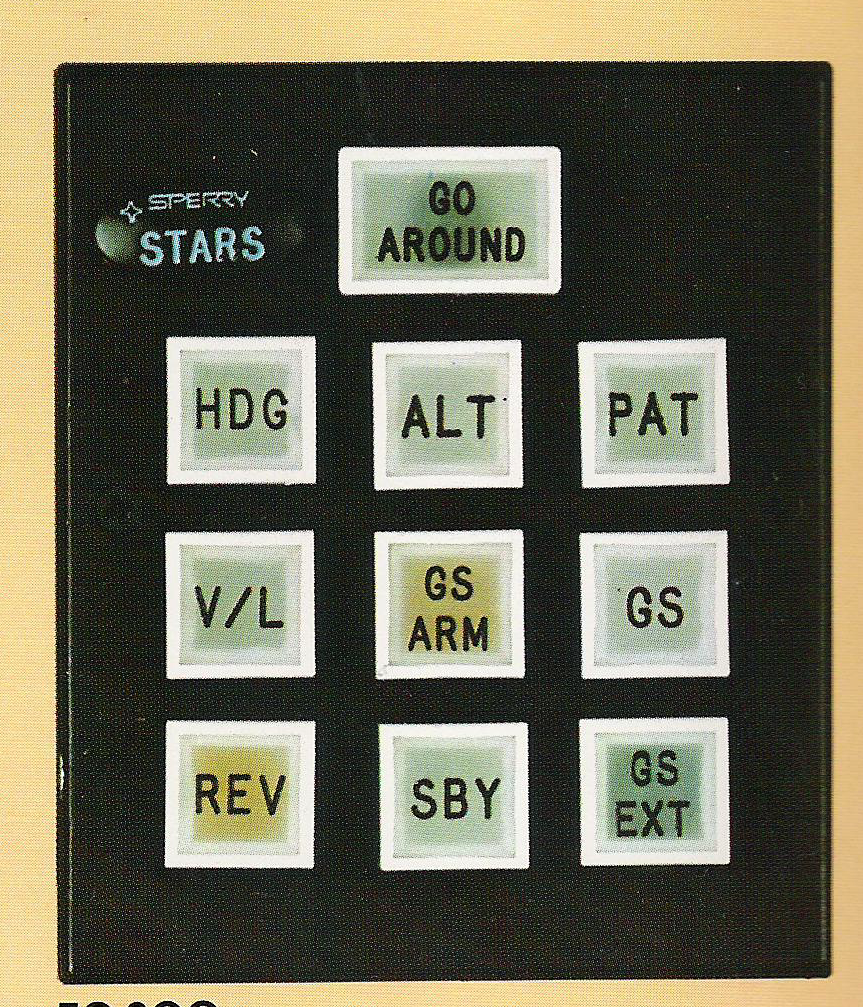
\includegraphics[width=0.6\textwidth]{07.directores.y.ctrol.automatico.vuelo/imagenes/computadora_sperry.png}  
  \caption{Imagen Computadora de Control (gentileza Sperry)}
  \label{fig:07.computadora.sperry}
\end{figure}

\section{Modos de operaci\'on}
\label{sec:modos.operacion}

Este sistema utiliza los datos de VOR-Localizadores y de Senda de Planeo,
proporcionados por los receptores de navegaci\'on corrientes.
Utiliza tambi\'en datos de altitud de un sensor de altura barom\'etrico
propio (adem\'as del de sistema de radio-alt\'imetro), datos de rumbo
desde un gir\'oscopo direccional y de actitud desde un gir\'oscopo
vertical, elementos estos que pertenecen al mismo sistema.

Todas estas informaciones son computadas siendo finalmente enviado su
resultado a comandar las barras directoras del sistema para guiar al
piloto en las maniobras que debe efectuar, para mantener o tomar la
senda de vuelo selectada, tanto para la navegaci\'on como para la
aproximaci\'on de aterrizaje.

Los modos de operaci\'on que puede selectar el piloto son los siguientes:

  \begin{tabular}{lm{3mm}llm{3mm}l}
\rowcolor{cyan!10}
    	SBY &  & Preparado &
	GO AROUND &  & Escape \\
\rowcolor{yellow!10}
	ALT &  & Mantenimiento de altura    &
	PAT &  & Ajuste de actitud en cabeceo \\
\rowcolor{cyan!10}
	HDB &  & Rumbo selectado &
	V/L &  & VOR - Localizador \\
\rowcolor{yellow!10}
        GS ARM & & Armado Pendiente de Planeo &
	GS & & Pendiente de Planeo \\
\rowcolor{cyan!10}
	GS EXT & &  &
	REV & & Curso opuesto \\
  \end{tabular}

\subsection{Modo Preparado (SBY)}
\label{sec:modo.sby}
Mediante el mismo el sistema es puesto en condiciones de operar cuando sea
requerido y encontr\'andose las barras del ADI fuera de la vista,
operando \'este como un indicador de referencia de actitud.
Este sistema est\'a energizado si lo est\'a el sistema de corriente
alterna del avi\'on, por lo tanto permite la selecci\'on de cualquier modo siempre que las banderas de precauci\'on respectivas se encuentren fuera de la
vista.

Se selecciona el moto SBY presionando la tecla correspondiente
en tablero, al seleccionarla se iluminan los dem\'as modos
como prueba de l\'amparas y al soltarlo solo SBY queda iluminado.

Al seleccionarse otro modo las barras directoras responden a las salidas
de la computadora, luego el piloto debe ``volar'' el avi\'on en miniatura
del ADI hacia las barras directoras e interceptarlas. Al mantener esta
condici\'on ser\'an efectuadas las maniobras necesarias para interceptar
y/o mantener un curso deseado.

\subsection{Modo Ajuste Actitud de Cabeceo (Pitch Attitude Trim, PAT)}
\label{sec:modo.ajuste.pitch}

Permite selectar un \'angulo de trepada o descenso por medio de la perilla
de ajuste de ajuste de actitud de cabeceo, que se encuentra en el frente y
en el extremo inferior izquierdo
del ADI (Figura \ref{fig:07.adi.sperry}, Pitch attitude trim knob).

Al presionar PAT, debe mantenerse encendida la luz de dicho modo
para que se confirme el mismo, la barra de comando de cabeceo del
ADI se ubica de manera que el piloto tome la actitud de cabeceo
deseada.

El modo PAT puede ser utilizado con cualquier otro modo de 
control de alabeo (p.e. el HDG) pero
resulta incompatible con otros modos de cabeceo (p.e. GO AROUND, ALT).

Si la se\~nal de cabeceo se torna inv\'alida, la barra de comando saldr\'a 
de vista y el bot\'on del modo permanecer\'a iluminado.

\subsection{Modo Rumbo Selectado (Heading HDG)}
\label{sec:hdg}

Se utiliza para interceptar y mantener un rumbo de vuelo deseado.
Al presionar HDG se debe iluminar el bot\'on, confirmando la
operaci\'on del mismo.
Si el modo resultara no v\'alido, la barra de comando de alabeo
saldr\'a de vista pero el bot\'on continuar\'a iluminado.

Utilizando la perilla de rumbo selectado ubicada en  el
HSI (Figura \ref{fig:07.hsi.sperry}, Heading knob),
se posiciona el \'indice de rumbo selectado en el rumbo
deseado 
(Figura \ref{fig:07.hsi.sperry}, Heading bug). 
Este debe ser menor a 170º respecto al rumbo actual de la aeronave.

La computadora controlar\'a los movimientos de la barra de
alabeo en el ADI a fin de dirigir al piloto para corregir
el alabeo del avi\'on de forma de interseptar el curso elegido
sin sobrepasamiento.

Para prevenir actitudes extremas, la computadora limita los \'angulos
de alabeo a un m\'aximo de 30º.

Si el modo HDG es selectado desde el modo SBY, en el ADI s\'olo
aparecer\'a la barra de alabeo. 
Si el modo es selectado con el modo PAT o ALT, aparecer\'a adem\'as
la barra de cabeceo.

\subsection{Modo mantenimiento de altura (ALT)}
\label{sec:alt}

Brinda la posibilidad de mantener una altura barom\'etrica deseada,
la cual ser\'a la presente al momento de selectar este modo.

Entonces, se nivela la aeronave a la altura deseada y se oprime
el modo ALT, confirm\'andose su operaci\'on por permanecer el 
bot\'on iluminado.

La computadora brindar\'a la informaci\'on necesaria para
posicionar la barra de cabeceo en el ADI, de forma de 
que el piloto tome las actitudes necesarias para mantener
la altitud barom\'etrica deseada.

Para prevenir acciones extremas, el comando del \'angulo de
cabeceo est\'a limitado a $\mp$ 10º.

En caso de alg\'un mal funcionamiento, la barra directora
de cabeceo en el ADI saldr\'a de vista y la luz de ALT
se apagar\'a en el teclado.

Adem\'as, a los efectos de proteger el elemento sensor de altura,
el modo se cancelar\'a al producirse un cambio sustancial respecto
a la altura selectada, desapareciendo la barra de control
de cabeceo.
Por ejemplo, al desviarse a nivel del mar en $\mp$ 400 pies (120 m)
o en $\mp$ 1200 pies (360 m) a 40000 pies (12000 m) de altura. 


\subsection{Modo Escape (GO AROUND)}
\label{sec:go.araund}

Este modo cancela todos los otros modos y provee un comando de trepada
prefijado, juntamente con un comando de nivelaci\'on de las alas.

El modo GO AROUND se selecta presionando el bot\'on correspondiente
sobre el teclado de la computadora o mediante un bot\'on en el
volante de mando.

En ocasi\'on de una aproximaci\'on fallida, se selecta este modo
indicando las barras del ADI la actitud a tomar.

Si el gir\'oscopo vertical asociado al sistema entrega datos
incorrectos o no v\'alidos, las barras en el ADI salen de
la vista mientras que el bot\'on GO AROUND permanecer\'a iluminado.


\subsection{Modo VOR - Localizador (V/L)}
\label{sec:V_L}

Permite mediante la barra de alabeo del ADI, interceptar y mantener
un rumbo deseado, operaci\'on que se efectuar\'a suavemente
limitando la computadora los \'angulos de alabeo a $\mp$ 30º.

\subsection{Armado Pendiente de Planeo}
\label{sec:GS.arm}

Por medio de este modo se prepara al sistema para la captura
autom\'atica del haz de pendiente de planeo 
cuando el avi\'on se aproxime al centro del haz de pendiente
de planeo desde abajo de \'este, si el avi\'on se encuentra
por arriba la luz del bot\'on GS-ARM se apagar\'a y la
computadora activar\'a autom\'aticamente el modo GS.

\subsection{Pendiente de Planeo}
\label{sec:gs}

Permite al piloto efectuar la captura de la pendiente de planeo
desde arriba o abajo del haz. La barra de mando de cabeceo mostrar\'a
la actitud a tomar, se encuentre el avi\'on arriba o abajo de la pendiente
de planeo.
La computadora limita los \'angulos de cabeceo a $\mp$ 10º aproximadamente.
La barra de mando de alabeo permitir\'a mantener la l\'inea central del
localizador.

\subsection{Modo anunciador ampliaci\'on de indicaci\'on en pendiente de planeo (GS EXT)}
\label{sec:gs.ext}

Provee un ajuste autom\'atico de ganancia para compensar el estrechamiento
del haz de pendiente de planeo, \'este modo es enganchado
autom\'aticamente al detectarse el marcador medio o a los 250 pies (76,2 m)
de altura.

\subsection{Modo Curso Opuesto (REV)}
\label{sec:rev}

Este modo da la posibilidad de volar el curso de localizador opuesto.

\section{Incorporaci\'on del sistema de radioalt\'imetro}
\label{sec:incorporacion.sistema.radio.altimetro}

El radioalt\'imetro provee una indicaci\'on de altura absoluta en un indicador,
pero adem\'as se interconecta con el director de vuelo a los fines
de manejar la barra de radioaltura en el ADI.

Cuando el sistema de radioalt\'imetro funciona, la barra de radioaltura aparece a la vista
en la parte inferior del instrumento a los 61 (sesenta y un) metros y, a medida que
el avi\'on se acerca a tierra, esta barra sube simulando el acercamiento de la aeronave
a tierra mediante el acercamiento relativo del avi\'on miniatura del ADI
a la barra en miniatura que simula el terreno.

Al tocar tierra la aeronave, la barra de altura del instrumento toca la parte
inferior del avi\'on simb\'olico del ADI.

El sistema de radioaltimetro est\'a compuesto por dos (2) antenas, una transmisora
y otra receptora, un transceptor y un indicador.
Su principio de funcionamiento se basa en la emisi\'on de ondas de UHF, moduladas
en frecuencia, por la antena transmisora, las cuales son reflejadas por la superficie
terrestre y receptadas por la segunda antena. La diferencia de frecuencia entre
las ondas emitidas y las reflejadas es representativa de la altura a la cual se
encuentra la aeronave del suelo, y es indicada en el instrumento.

En otros sistemas se utiliza la modulaci\'on de pulsos.


\section{Integraci\'on con el Sistema de Piloto Autom\'atico}
\label{sec:07.AFCS}

El \ac{AFCS} provee la integraci\'on del \ac{FDS} con el Piloto Autom\'atico, este sistema se encuentra habitualmente en aeronaves de alta performance pero debido a los avances en procesamiento digital se encuentran actualmente disponibles para aviaci\'on general.

En algunos de estos sistemas son tan avanzados que permiten extender la programaci\'on, el nivel de integraci\'on con las ayudas, integraci\'on con sistemas de control de motor y combinar todo esto en una \'unica
consola con interfaz para el usuario.

\begin{tcolorbox}

 Ejemplo de implementaci\'on de un \ac{AFCS} puede consultarse en el siguiente documento 
  \href{http://www.smartcockpit.com/docs/Bombardier_CRJ_200-Automatic_Flight_Control_System.pdf}{Canadair
    Regional Jet 100/200 - Automatic Flight Control System}.

Otro ejemplo puede encontrarse en la siguiente publicaci\'on
\href{https://static.garmincdn.com/pumac/190-00498-07_0A_Web.pdf}{Gu\'ia del piloto del sistema Garmin G1000 Integrated Flight Deck}

\end{tcolorbox}

A su vez los \ac{AFCS} pueden integrarse con los \ac{AHRS} y ayudas para la navegaci\'on incluyendo senda de planeo. 

\subsection{\ac{AHRS}}
\label{sec:07.AHRS}


Una notable mejora a los tradicionales sistemas giroscópicos vino dada por las Unidades de Medición Inercial, en ingl\'es \ac{IMU}, las cuales consisten en dispositivos que utilizando una combinación de acelerómetros y giróscopos, permiten determinar la velocidad, orientación y fuerzas gravitacionales de una aeronave.
Estas unidades constituyeron el elemento principal de los \ac{INS} empleados  en los primeros ``\emph{glass cockpits}'' en la aviaci\'on militar y comercial. Su coste era muy elevado para la aviación general por lo que  se continuaron utilizando los sistemas anteriores en esta rama.

Las \ac{IMU} presentan acumulación de errores durante su utilización,  puesto que el sistema de guiado está continuamente integrando la aceleración para calcular la velocidad y la posición, los errores de medición se acumulan (deriva).

Es aqu\'i cuando aparecen las \ac{AHRS} que brindaron un  avance notable sobre las \ac{IMU}, puesto que fueron creados para proporcionar una mayor fiabilidad y precisión. Estos sistemas consisten,  básicamente, en una serie de sensores en los tres ejes coordenados a partir de los cuales se obtiene la información de rumbo y actitud de la aeronave.
De esta forma, un AHRS proporciona al piloto orientación tridimensional mediante la integración de gir\'oscoos y la combinación de los datos obtenidos mediante acelerómetros y magnetómetros. 
Debe señalarse que los gir\'oscopos utilizados por los AHRS son muy diferentes de los tradicionales ya que, al igual que los acelerómetros y los magnetómetros, se trata de Sistemas Microelectromecánicos, en ingl\'es \ac{MEMS}. 

Los \ac{MEMS}  pueden definirse como componentes mecánicos y electromecánicos miniaturizados, su desarrollo comenz\'o a mediados de los a\~nos 1980. Para su desarrollo se utilizan técnicas de microfabricación similares a las empleadas en la producción de circuitos integrados. Estos dispositivos  están constituidos por estructuras con tamaños típicos entre 1 y 100 $\mu$m.

A fin de tener en cuenta la deriva que  puede producir datos erróneos, los sistemas AHRS utilizan acelerómetros y magnetómetros. El acelerómetro hace uso de la gravedad para servir tanto de referencia inicial de actitud como de referencia en vuelo. Por su parte, el magnetómetro utiliza el campo magnético de la tierra para proporcionar información de rumbo. Finalmente, el AHRS agrega toda la información de estos diferentes componentes y lleva a cabo complejos cálculos mediante los algoritmos convenientes para proporcionar datos de actitud y rumbo de gran fiabilidad.



Los \ac{AHRS}
 están espec\'ificamente dise\~nados para reemplazar a los antiguos instrumentos de control girosc\'opico y proporcionar una mejor precisi\'on y fiabilidad. 


Usualmente los \ac{AHRS} están conformados por gir\'oscopos de estado s\'olido o sistemas microelectromecánicos, aceler\'ometros, y magnetómetros que proporcionan datos seg\'un los tres ejes del espacio. 


Algunos \ac{AHRS} utilizan receptores \ac{GPS} para mejorar la estabilidad a largo plazo de los gir\'oscopos. 
%Como técnica de fusión sensorial, es habitual emplear Filtros de Kalman, de tal manera que se obtenga una única solución a partir de las diversas fuentes de datos originales. 
La diferencia entre estos sistemas con los  \ac{INS} en que se basan en el uso de magnet\'ometros y/o receptores \ac{GPS} para corregir los datos en bruto brindados por los  gir\'oscopos.




\begin{tcolorbox}
  Los \ac{AHRS} han demostrado ser altamente fiables y se emplean
  tanto en aeronaves comerciales como privadas e incluso UAVs.

  % Recientes avances en la fabricación de sistemas
  % microelectromecánicos, han hecho que el precio de AHRS
  % certificados por la FAA de Estados Unidos esté por debajo de los
  % U\$15000 .
  Como ejemplo de un sistema \ac{AHRS} puede consultarse el
  \href{http://www.archangel.com/images/documents/ahr50/AHR50Overview.pdf}{AHR50
    de la empresa Archangel Systems Inc.}
o el
\href{https://watson-gyro.com/wp-content/uploads/delightful-downloads/2018/03/AHRS-E304-Spec-Sheet.pdf}{AHRS-E304 de la empresa Watson Industries Inc.}

Un ejemplo de \ac{AHRS} peque\~no es el 
\href{https://www.microstrain.com/inertial/3DM-GX5-25}{3DM-GX5-25 AHRS de la empresa Parker Lord.}
\end{tcolorbox}

\begin{tcolorbox}
  Los AHRS se integran normalmente en los \ac{EFIS}, combin\'andose
  con Computadoras de Datos de Aire por lo que se los suele denominan
  \ac{ADAHRS}, de esta manera proporcionan información adicional como
  la velocidad de la aeronave relativa al aire, altitud y temperatura
  del aire en el exterior.

  Como ejemplo de un sistema \ac{ADAHRS} puede consultarse el 
  \href{http://www.archangel.com/images/documents/ahr150/AHR150overview.pdf}{AHR150A/300A de la empresa Archangel Systems Inc.}
\end{tcolorbox}





% \section{Indicador director de actitud, Indicador de situación horizontal}
% \label{sec:U07.01.HSI}

                         
% \section{Componentes y modos del director de vuelo, diagrama en bloque, flujo de señales}
% \label{sec:U07.02.director.vuelo}

          
% \section{Piloto automático, componentes, diagrama en bloque, funcionamiento en los distintos modos}
% \label{sec:U07.03.piloto.automatico}


%--------------LINKS A BIBLIOGRAFIA HISTORICA

% \href{https://cdn.rochesteravionicarchives.co.uk/img/catalog/ZZ_1357579863_DDBR0186+%28O%26A-1b%29.pdf}{The Concorde automatic flight control system}

% \href{https://cdn.rochesteravionicarchives.co.uk/img/catalog/2_D0584.pdf}{VC10 Flight Control System. Parte I}
% \href{https://cdn.rochesteravionicarchives.co.uk/img/catalog/2_D0584_%28A-1b%29.pdf}{VC10 Flight Control System. Parte II}

% \href{https://cdn.rochesteravionicarchives.co.uk/img/catalog/ZZ_1376766417_DDBR0300+%28O%26A-1b%29.pdf}{The Design and Development of the M RCA Autopilot}


Un caso interesante de sistema Fly-By-Wire ocurrió con el primer prototipo del X-31

% En el siguiente \href{Video}{https://www.youtube.com/watch?v=x1E3xpePbmA&feature=emb_logo}
% se cuenta la historia del suceso y la cadena de errores cometidos.